% Options for packages loaded elsewhere
\PassOptionsToPackage{unicode}{hyperref}
\PassOptionsToPackage{hyphens}{url}
%
\documentclass[
]{article}
\usepackage{lmodern}
\usepackage{amssymb,amsmath}
\usepackage{ifxetex,ifluatex}
\ifnum 0\ifxetex 1\fi\ifluatex 1\fi=0 % if pdftex
  \usepackage[T1]{fontenc}
  \usepackage[utf8]{inputenc}
  \usepackage{textcomp} % provide euro and other symbols
\else % if luatex or xetex
  \usepackage{unicode-math}
  \defaultfontfeatures{Scale=MatchLowercase}
  \defaultfontfeatures[\rmfamily]{Ligatures=TeX,Scale=1}
\fi
% Use upquote if available, for straight quotes in verbatim environments
\IfFileExists{upquote.sty}{\usepackage{upquote}}{}
\IfFileExists{microtype.sty}{% use microtype if available
  \usepackage[]{microtype}
  \UseMicrotypeSet[protrusion]{basicmath} % disable protrusion for tt fonts
}{}
\makeatletter
\@ifundefined{KOMAClassName}{% if non-KOMA class
  \IfFileExists{parskip.sty}{%
    \usepackage{parskip}
  }{% else
    \setlength{\parindent}{0pt}
    \setlength{\parskip}{6pt plus 2pt minus 1pt}}
}{% if KOMA class
  \KOMAoptions{parskip=half}}
\makeatother
\usepackage{xcolor}
\IfFileExists{xurl.sty}{\usepackage{xurl}}{} % add URL line breaks if available
\IfFileExists{bookmark.sty}{\usepackage{bookmark}}{\usepackage{hyperref}}
\hypersetup{
  pdftitle={UMAP EDA},
  pdfauthor={Niklas Rindtorff},
  hidelinks,
  pdfcreator={LaTeX via pandoc}}
\urlstyle{same} % disable monospaced font for URLs
\usepackage[margin=1in]{geometry}
\usepackage{color}
\usepackage{fancyvrb}
\newcommand{\VerbBar}{|}
\newcommand{\VERB}{\Verb[commandchars=\\\{\}]}
\DefineVerbatimEnvironment{Highlighting}{Verbatim}{commandchars=\\\{\}}
% Add ',fontsize=\small' for more characters per line
\usepackage{framed}
\definecolor{shadecolor}{RGB}{248,248,248}
\newenvironment{Shaded}{\begin{snugshade}}{\end{snugshade}}
\newcommand{\AlertTok}[1]{\textcolor[rgb]{0.94,0.16,0.16}{#1}}
\newcommand{\AnnotationTok}[1]{\textcolor[rgb]{0.56,0.35,0.01}{\textbf{\textit{#1}}}}
\newcommand{\AttributeTok}[1]{\textcolor[rgb]{0.77,0.63,0.00}{#1}}
\newcommand{\BaseNTok}[1]{\textcolor[rgb]{0.00,0.00,0.81}{#1}}
\newcommand{\BuiltInTok}[1]{#1}
\newcommand{\CharTok}[1]{\textcolor[rgb]{0.31,0.60,0.02}{#1}}
\newcommand{\CommentTok}[1]{\textcolor[rgb]{0.56,0.35,0.01}{\textit{#1}}}
\newcommand{\CommentVarTok}[1]{\textcolor[rgb]{0.56,0.35,0.01}{\textbf{\textit{#1}}}}
\newcommand{\ConstantTok}[1]{\textcolor[rgb]{0.00,0.00,0.00}{#1}}
\newcommand{\ControlFlowTok}[1]{\textcolor[rgb]{0.13,0.29,0.53}{\textbf{#1}}}
\newcommand{\DataTypeTok}[1]{\textcolor[rgb]{0.13,0.29,0.53}{#1}}
\newcommand{\DecValTok}[1]{\textcolor[rgb]{0.00,0.00,0.81}{#1}}
\newcommand{\DocumentationTok}[1]{\textcolor[rgb]{0.56,0.35,0.01}{\textbf{\textit{#1}}}}
\newcommand{\ErrorTok}[1]{\textcolor[rgb]{0.64,0.00,0.00}{\textbf{#1}}}
\newcommand{\ExtensionTok}[1]{#1}
\newcommand{\FloatTok}[1]{\textcolor[rgb]{0.00,0.00,0.81}{#1}}
\newcommand{\FunctionTok}[1]{\textcolor[rgb]{0.00,0.00,0.00}{#1}}
\newcommand{\ImportTok}[1]{#1}
\newcommand{\InformationTok}[1]{\textcolor[rgb]{0.56,0.35,0.01}{\textbf{\textit{#1}}}}
\newcommand{\KeywordTok}[1]{\textcolor[rgb]{0.13,0.29,0.53}{\textbf{#1}}}
\newcommand{\NormalTok}[1]{#1}
\newcommand{\OperatorTok}[1]{\textcolor[rgb]{0.81,0.36,0.00}{\textbf{#1}}}
\newcommand{\OtherTok}[1]{\textcolor[rgb]{0.56,0.35,0.01}{#1}}
\newcommand{\PreprocessorTok}[1]{\textcolor[rgb]{0.56,0.35,0.01}{\textit{#1}}}
\newcommand{\RegionMarkerTok}[1]{#1}
\newcommand{\SpecialCharTok}[1]{\textcolor[rgb]{0.00,0.00,0.00}{#1}}
\newcommand{\SpecialStringTok}[1]{\textcolor[rgb]{0.31,0.60,0.02}{#1}}
\newcommand{\StringTok}[1]{\textcolor[rgb]{0.31,0.60,0.02}{#1}}
\newcommand{\VariableTok}[1]{\textcolor[rgb]{0.00,0.00,0.00}{#1}}
\newcommand{\VerbatimStringTok}[1]{\textcolor[rgb]{0.31,0.60,0.02}{#1}}
\newcommand{\WarningTok}[1]{\textcolor[rgb]{0.56,0.35,0.01}{\textbf{\textit{#1}}}}
\usepackage{graphicx,grffile}
\makeatletter
\def\maxwidth{\ifdim\Gin@nat@width>\linewidth\linewidth\else\Gin@nat@width\fi}
\def\maxheight{\ifdim\Gin@nat@height>\textheight\textheight\else\Gin@nat@height\fi}
\makeatother
% Scale images if necessary, so that they will not overflow the page
% margins by default, and it is still possible to overwrite the defaults
% using explicit options in \includegraphics[width, height, ...]{}
\setkeys{Gin}{width=\maxwidth,height=\maxheight,keepaspectratio}
% Set default figure placement to htbp
\makeatletter
\def\fps@figure{htbp}
\makeatother
\setlength{\emergencystretch}{3em} % prevent overfull lines
\providecommand{\tightlist}{%
  \setlength{\itemsep}{0pt}\setlength{\parskip}{0pt}}
\setcounter{secnumdepth}{-\maxdimen} % remove section numbering

\title{UMAP EDA}
\author{Niklas Rindtorff}
\date{}

\begin{document}
\maketitle

\begin{Shaded}
\begin{Highlighting}[]
\KeywordTok{library}\NormalTok{(ggplot2)}
\KeywordTok{library}\NormalTok{(dplyr)}
\KeywordTok{library}\NormalTok{(tidyr)}
\KeywordTok{library}\NormalTok{(magrittr)}
\KeywordTok{library}\NormalTok{(purrr)}
\KeywordTok{library}\NormalTok{(readr)}
\KeywordTok{library}\NormalTok{(here)}
\KeywordTok{library}\NormalTok{(tibble)}
\KeywordTok{library}\NormalTok{(ggrastr)}
\KeywordTok{library}\NormalTok{(cowplot)}
\KeywordTok{library}\NormalTok{(princurve)}
\KeywordTok{library}\NormalTok{(scico)}
\KeywordTok{library}\NormalTok{(ggridges)}
\KeywordTok{library}\NormalTok{(cowplot)}
\KeywordTok{library}\NormalTok{(tibble)}
\KeywordTok{library}\NormalTok{(grDevices)}
\KeywordTok{library}\NormalTok{(stats)}

\CommentTok{# parameter}
\KeywordTok{print}\NormalTok{(}\StringTok{"parameter input:"}\NormalTok{)}
\end{Highlighting}
\end{Shaded}

\begin{verbatim}
## [1] "parameter input:"
\end{verbatim}

\begin{Shaded}
\begin{Highlighting}[]
\KeywordTok{print}\NormalTok{(params}\OperatorTok{$}\NormalTok{data)}
\end{Highlighting}
\end{Shaded}

\begin{verbatim}
## [1] "data/processed/morphology/umap_absolute_all_drugs_sampled.Rds"
\end{verbatim}

\begin{Shaded}
\begin{Highlighting}[]
\KeywordTok{print}\NormalTok{(params}\OperatorTok{$}\NormalTok{data_harmony)}
\end{Highlighting}
\end{Shaded}

\begin{verbatim}
## [1] "data/processed/morphology/harmony_umap_absolute_all_drugs_sampled.Rds"
\end{verbatim}

\hypertarget{introduction}{%
\section{Introduction}\label{introduction}}

After extracting features from segmented organoids, we are interested in
a set of questions regarding (I) morphological differences between
organoid lines, (II) robust morphological states across organoid lines
and (III) how such states correlate to biological organoid state by
means of gene expression, drug perturbation etc.

The current preprocessing of our data includes: * filtering of objects
below 300 pixels * removing objects touching the original image boundary
* initial filtering of blurry organoids using a supervised random-forest
classifier * normalization of organoid features to each plate's
distribution

Further, we added the following steps: * we remove noisy features and
reduce data dimensionality using PCA, we keep 25 components (arbitrary
cutoff) * ( we experiment with \emph{Harmony}, a method to remove batch
effects in high dimensional data, such as single-cell RNA-Seq data) * we
perform a UMAP projection of the complete data

In this vignette we are interested in the overall structure of the
embedding and the effect of \emph{Harmony}. We compare pre-processed
data run through \emph{Harmony} with data that was directly projected
using UMAP.

\begin{Shaded}
\begin{Highlighting}[]
\NormalTok{organoid_morphology <-}\StringTok{ }\KeywordTok{read_delim}\NormalTok{(here}\OperatorTok{::}\KeywordTok{here}\NormalTok{(}\StringTok{"references/imaging/visual_classification_organoids.csv"}\NormalTok{), }\StringTok{";"}\NormalTok{, }\DataTypeTok{escape_double =} \OtherTok{FALSE}\NormalTok{, }\DataTypeTok{trim_ws =} \OtherTok{TRUE}\NormalTok{) }\OperatorTok\StringTok{ }
\StringTok{  }\NormalTok{dplyr}\OperatorTok{::}\KeywordTok{select}\NormalTok{(}\DataTypeTok{line =}\NormalTok{ organoid, }\DataTypeTok{morphology =}\NormalTok{ visual_inspection_v2) }\OperatorTok\StringTok{ }
\StringTok{  }\KeywordTok{expand_grid}\NormalTok{(., }\DataTypeTok{version =} \KeywordTok{c}\NormalTok{(}\StringTok{"01"}\NormalTok{, }\StringTok{"02"}\NormalTok{)) }\OperatorTok
\StringTok{  }\KeywordTok{mutate}\NormalTok{(}\DataTypeTok{line =} \KeywordTok{paste0}\NormalTok{(line, version)) }\OperatorTok\StringTok{ }
\StringTok{  }\NormalTok{dplyr}\OperatorTok{::}\KeywordTok{select}\NormalTok{(}\OperatorTok{-}\NormalTok{version)}

\NormalTok{umap_sampled <-}\StringTok{ }\KeywordTok{read_rds}\NormalTok{(here}\OperatorTok{::}\KeywordTok{here}\NormalTok{(params}\OperatorTok{$}\NormalTok{data)) }\OperatorTok\StringTok{ }\KeywordTok{left_join}\NormalTok{(organoid_morphology)}
\NormalTok{umap_sampled_h <-}\StringTok{ }\KeywordTok{read_rds}\NormalTok{(here}\OperatorTok{::}\KeywordTok{here}\NormalTok{(params}\OperatorTok{$}\NormalTok{data_harmony)) }\OperatorTok\StringTok{ }\KeywordTok{left_join}\NormalTok{(organoid_morphology)}

\CommentTok{# umap_df <- rbind(pca_df_raw %>% mutate(status = "raw"),}
\CommentTok{#                 pca_df_harmony %>% mutate(status = "harmony"))}
\end{Highlighting}
\end{Shaded}

\hypertarget{organoid-size}{%
\section{Organoid Size}\label{organoid-size}}

The central cluster contains mostly large organoids, while two seperate
clusters contain smaller objects.

\begin{Shaded}
\begin{Highlighting}[]
\NormalTok{umap_size <-}\StringTok{ }\ControlFlowTok{function}\NormalTok{(umap, main)\{}
\NormalTok{  umap }\OperatorTok
\StringTok{  }\CommentTok{#filter(Size < 1000) %>%}
\StringTok{  }\KeywordTok{ggplot}\NormalTok{(}\KeywordTok{aes}\NormalTok{(v1, v2, }\DataTypeTok{color =}\NormalTok{ size_log)) }\OperatorTok{+}\StringTok{ }
\StringTok{  }\KeywordTok{geom_point_rast}\NormalTok{(}\DataTypeTok{alpha =} \FloatTok{0.5}\NormalTok{, }\DataTypeTok{size =} \FloatTok{0.35}\NormalTok{) }\OperatorTok{+}\StringTok{ }
\StringTok{  }\KeywordTok{scale_color_viridis_c}\NormalTok{() }\OperatorTok{+}
\StringTok{  }\KeywordTok{theme_cowplot}\NormalTok{() }\OperatorTok{+}
\StringTok{  }\KeywordTok{labs}\NormalTok{(}\DataTypeTok{x =} \StringTok{"UMAP 1"}\NormalTok{,}
       \DataTypeTok{y =} \StringTok{"UMAP 2"}\NormalTok{,}
       \DataTypeTok{title =}\NormalTok{ main,}
       \DataTypeTok{color =} \StringTok{"ln(size)"}\NormalTok{) }\OperatorTok{+}\StringTok{ }
\StringTok{  }\KeywordTok{theme}\NormalTok{(}\DataTypeTok{legend.position =} \StringTok{"bottom"}\NormalTok{)}
\NormalTok{\}}

\NormalTok{p1 <-}\StringTok{ }\KeywordTok{umap_size}\NormalTok{(umap_sampled_h, }\StringTok{"Harmony normalised, All data"}\NormalTok{)}
\NormalTok{p2 <-}\StringTok{ }\KeywordTok{umap_size}\NormalTok{(umap_sampled, }\StringTok{"Raw Data, All data"}\NormalTok{)}
\CommentTok{# p3 <- umap_size(umap_sampled_dmso_h, "Harmony normalised, DMSO")}
\CommentTok{# p4 <- umap_size(umap_sampled_dmso, "Raw Data, DMSO")}

\KeywordTok{plot_grid}\NormalTok{(}
\NormalTok{  p1, p2,}
\CommentTok{#  p3, p4,}
  \DataTypeTok{labels =} \StringTok{"AUTO"}\NormalTok{, }\DataTypeTok{ncol =} \DecValTok{2}
\NormalTok{) }\OperatorTok{+}\StringTok{  }\KeywordTok{ggsave}\NormalTok{(here}\OperatorTok{::}\KeywordTok{here}\NormalTok{(}\StringTok{"reports/gg_size_panel.pdf"}\NormalTok{), }
            \DataTypeTok{width =} \DecValTok{8}\NormalTok{,}
            \DataTypeTok{height =} \DecValTok{4}\NormalTok{)}
\end{Highlighting}
\end{Shaded}

\includegraphics{2.0-nr-embedding_inspection_files/figure-latex/unnamed-chunk-3-1.pdf}

\hypertarget{organoid-viability}{%
\section{Organoid Viability}\label{organoid-viability}}

\begin{Shaded}
\begin{Highlighting}[]
\NormalTok{umap_ldc <-}\StringTok{ }\ControlFlowTok{function}\NormalTok{(umap, main)\{}
\NormalTok{  umap }\OperatorTok
\StringTok{  }\CommentTok{#filter(Size < 1000) %>%}
\StringTok{  }\KeywordTok{ggplot}\NormalTok{(}\KeywordTok{aes}\NormalTok{(v1, v2, }\DataTypeTok{color =}\NormalTok{ prob_dead)) }\OperatorTok{+}\StringTok{ }
\StringTok{  }\KeywordTok{geom_point_rast}\NormalTok{(}\DataTypeTok{alpha =} \FloatTok{0.5}\NormalTok{, }\DataTypeTok{size =} \FloatTok{0.35}\NormalTok{) }\OperatorTok{+}\StringTok{ }
\StringTok{  }\KeywordTok{scale_color_scico}\NormalTok{(}\DataTypeTok{palette =} \StringTok{'lajolla'}\NormalTok{) }\OperatorTok{+}\StringTok{ }\CommentTok{#lajolla #vikO}
\StringTok{  }\KeywordTok{theme_cowplot}\NormalTok{() }\OperatorTok{+}
\StringTok{  }\KeywordTok{labs}\NormalTok{(}\DataTypeTok{x =} \StringTok{"UMAP 1"}\NormalTok{,}
       \DataTypeTok{y =} \StringTok{"UMAP 2"}\NormalTok{,}
       \DataTypeTok{title =}\NormalTok{ main,}
       \DataTypeTok{color =} \StringTok{"p(dead)"}\NormalTok{) }\OperatorTok{+}\StringTok{ }
\StringTok{  }\KeywordTok{theme}\NormalTok{(}\DataTypeTok{legend.position =} \StringTok{"bottom"}\NormalTok{) }\OperatorTok{+}\StringTok{ }
\StringTok{  }\KeywordTok{guides}\NormalTok{(}\DataTypeTok{fill =} \KeywordTok{guide_colourbar}\NormalTok{(}\DataTypeTok{barwidth =} \FloatTok{0.5}\NormalTok{, }\DataTypeTok{barheight =} \DecValTok{10}\NormalTok{))}
\NormalTok{\}}

\NormalTok{p1 <-}\StringTok{ }\KeywordTok{umap_ldc}\NormalTok{(umap_sampled_h, }\StringTok{"Harmony normalised, All data"}\NormalTok{)}
\NormalTok{p2 <-}\StringTok{ }\KeywordTok{umap_ldc}\NormalTok{(umap_sampled, }\StringTok{"Raw Data, All data"}\NormalTok{)}
\CommentTok{# p3 <- umap_ldc(umap_sampled_dmso_h, "Harmony normalised, DMSO")}
\CommentTok{# p4 <- umap_ldc(umap_sampled_dmso, "Raw Data, DMSO")}


\KeywordTok{plot_grid}\NormalTok{(}
\NormalTok{  p1, p2,}
\CommentTok{#  p3, p4,}
  \DataTypeTok{labels =} \StringTok{"AUTO"}\NormalTok{, }\DataTypeTok{ncol =} \DecValTok{2}
\NormalTok{) }\OperatorTok{+}\StringTok{  }\KeywordTok{ggsave}\NormalTok{(here}\OperatorTok{::}\KeywordTok{here}\NormalTok{(}\StringTok{"gg_ldc_panel.pdf"}\NormalTok{),}
            \DataTypeTok{width =} \DecValTok{8}\NormalTok{,}
            \DataTypeTok{height =} \DecValTok{4}\NormalTok{)}
\end{Highlighting}
\end{Shaded}

\includegraphics{2.0-nr-embedding_inspection_files/figure-latex/unnamed-chunk-4-1.pdf}

\begin{Shaded}
\begin{Highlighting}[]
\CommentTok{#p2 +  ggsave(paste0(PATH, "notebooks/PhenotypeSpectrum/gg_ldc.pdf"), width = 4, height = 4)}
\end{Highlighting}
\end{Shaded}

\begin{Shaded}
\begin{Highlighting}[]
\NormalTok{umap_morph <-}\StringTok{ }\ControlFlowTok{function}\NormalTok{(umap, main)\{}
\NormalTok{  umap }\OperatorTok
\StringTok{  }\CommentTok{#filter(Size < 1000) %>%}
\StringTok{  }\KeywordTok{ggplot}\NormalTok{(}\KeywordTok{aes}\NormalTok{(v1, v2, }\DataTypeTok{color =}\NormalTok{ morphology)) }\OperatorTok{+}\StringTok{ }
\StringTok{  }\KeywordTok{geom_point_rast}\NormalTok{(}\DataTypeTok{alpha =} \FloatTok{0.5}\NormalTok{, }\DataTypeTok{size =} \FloatTok{0.35}\NormalTok{) }\OperatorTok{+}\StringTok{ }
\StringTok{  }\KeywordTok{scale_color_brewer}\NormalTok{(}\DataTypeTok{type =} \StringTok{"qual"}\NormalTok{) }\OperatorTok{+}\StringTok{ }\CommentTok{#lajolla #vikO}
\StringTok{  }\KeywordTok{theme_cowplot}\NormalTok{() }\OperatorTok{+}
\StringTok{  }\KeywordTok{labs}\NormalTok{(}\DataTypeTok{x =} \StringTok{"UMAP 1"}\NormalTok{,}
       \DataTypeTok{y =} \StringTok{"UMAP 2"}\NormalTok{,}
       \DataTypeTok{title =}\NormalTok{ main) }\OperatorTok{+}\StringTok{ }
\StringTok{  }\KeywordTok{theme}\NormalTok{(}\DataTypeTok{legend.position =} \StringTok{"bottom"}\NormalTok{)}
\NormalTok{\}}

\NormalTok{p1 <-}\StringTok{ }\KeywordTok{umap_morph}\NormalTok{(umap_sampled_h, }\StringTok{"Harmony normalised, All data"}\NormalTok{)}
\NormalTok{p2 <-}\StringTok{ }\KeywordTok{umap_morph}\NormalTok{(umap_sampled, }\StringTok{"Raw Data, All data"}\NormalTok{)}
\CommentTok{# p3 <- umap_morph(umap_sampled_dmso_h, "Harmony normalised, DMSO")}
\CommentTok{# p4 <- umap_morph(umap_sampled_dmso, "Raw Data, DMSO")}


\KeywordTok{plot_grid}\NormalTok{(}
\NormalTok{  p1, p2,}
\CommentTok{#  p3, p4,}
  \DataTypeTok{labels =} \StringTok{"AUTO"}\NormalTok{, }\DataTypeTok{ncol =} \DecValTok{2}
\NormalTok{) }\OperatorTok{+}\StringTok{  }\KeywordTok{ggsave}\NormalTok{(here}\OperatorTok{::}\KeywordTok{here}\NormalTok{(}\StringTok{"gg_morph_panel.pdf"}\NormalTok{),}
            \DataTypeTok{width =} \DecValTok{8}\NormalTok{,}
            \DataTypeTok{height =} \DecValTok{4}\NormalTok{)}
\end{Highlighting}
\end{Shaded}

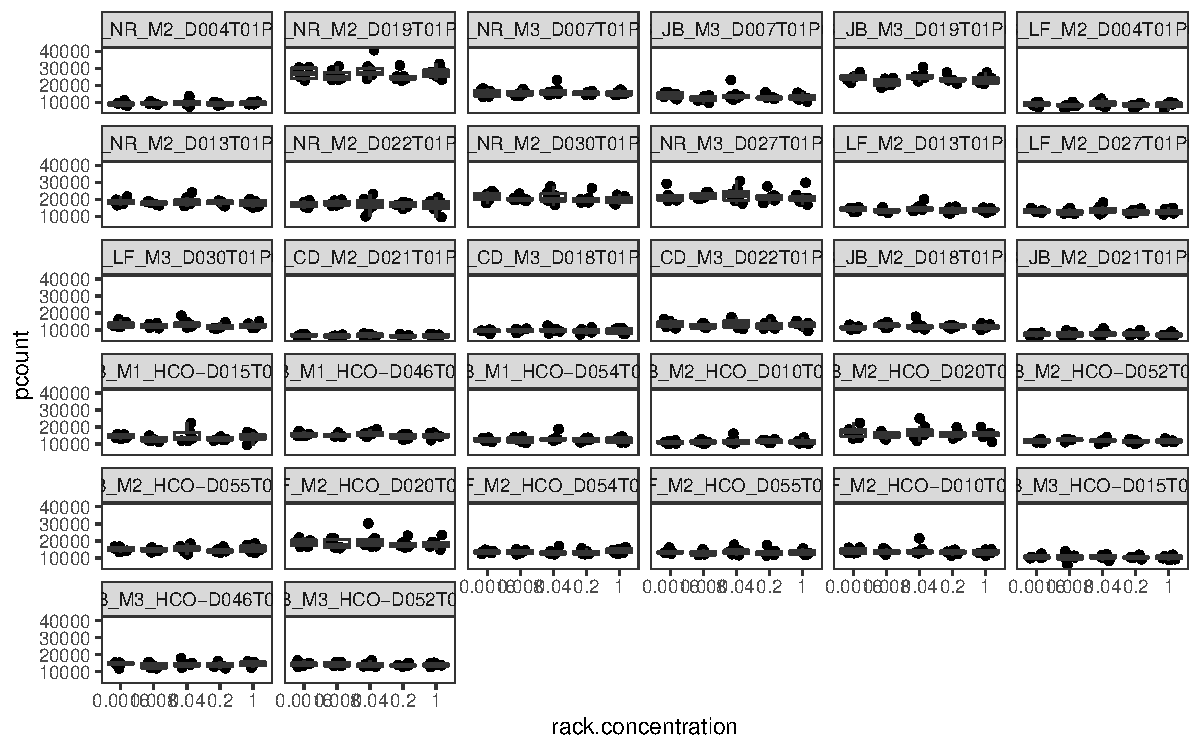
\includegraphics{2.0-nr-embedding_inspection_files/figure-latex/unnamed-chunk-5-1.pdf}

\begin{Shaded}
\begin{Highlighting}[]
\CommentTok{#p2 +  ggsave(paste0(PATH, "notebooks/PhenotypeSpectrum/gg_morph.pdf"))}
\end{Highlighting}
\end{Shaded}

\begin{Shaded}
\begin{Highlighting}[]
\NormalTok{umap_line <-}\StringTok{ }\ControlFlowTok{function}\NormalTok{(umap, main)\{}
\NormalTok{  umap }\OperatorTok
\StringTok{  }\CommentTok{#filter(Size < 1000) %>%}
\StringTok{  }\KeywordTok{ggplot}\NormalTok{(}\KeywordTok{aes}\NormalTok{(v1, v2, }\DataTypeTok{color =}\NormalTok{ line)) }\OperatorTok{+}\StringTok{ }
\StringTok{  }\KeywordTok{geom_point_rast}\NormalTok{(}\DataTypeTok{alpha =} \FloatTok{0.5}\NormalTok{, }\DataTypeTok{size =} \FloatTok{0.35}\NormalTok{) }\OperatorTok{+}\StringTok{ }
\StringTok{  }\KeywordTok{scale_color_brewer}\NormalTok{(}\DataTypeTok{type =} \StringTok{"qual"}\NormalTok{) }\OperatorTok{+}\StringTok{ }\CommentTok{#lajolla #vikO}
\StringTok{  }\KeywordTok{theme_cowplot}\NormalTok{() }\OperatorTok{+}
\StringTok{  }\KeywordTok{labs}\NormalTok{(}\DataTypeTok{x =} \StringTok{"UMAP 1"}\NormalTok{,}
       \DataTypeTok{y =} \StringTok{"UMAP 2"}\NormalTok{,}
       \DataTypeTok{title =}\NormalTok{ main) }\OperatorTok{+}\StringTok{ }
\StringTok{  }\KeywordTok{theme}\NormalTok{(}\DataTypeTok{legend.position =} \StringTok{"bottom"}\NormalTok{)}
\NormalTok{\}}

\NormalTok{p1 <-}\StringTok{ }\KeywordTok{umap_line}\NormalTok{(umap_sampled_h, }\StringTok{"Harmony normalised, All data"}\NormalTok{)}
\NormalTok{p2 <-}\StringTok{ }\KeywordTok{umap_line}\NormalTok{(umap_sampled, }\StringTok{"Raw Data, All data"}\NormalTok{)}
\CommentTok{# p3 <- umap_line(umap_sampled_dmso_h, "Harmony normalised, DMSO")}
\CommentTok{# p4 <- umap_line(umap_sampled_dmso, "Raw Data, DMSO")}


\KeywordTok{plot_grid}\NormalTok{(}
\NormalTok{  p1, p2,}
\CommentTok{#  p3, p4,}
  \DataTypeTok{labels =} \StringTok{"AUTO"}\NormalTok{, }\DataTypeTok{ncol =} \DecValTok{2}
\NormalTok{) }\OperatorTok{+}\StringTok{  }\KeywordTok{ggsave}\NormalTok{(here}\OperatorTok{::}\KeywordTok{here}\NormalTok{(}\StringTok{"gg_line_panel.pdf"}\NormalTok{),}
            \DataTypeTok{width =} \DecValTok{8}\NormalTok{,}
            \DataTypeTok{height =} \DecValTok{4}\NormalTok{)}

\CommentTok{#p2 +  ggsave(paste0(PATH, "notebooks/PhenotypeSpectrum/gg_line.pdf"))}
\end{Highlighting}
\end{Shaded}

\begin{Shaded}
\begin{Highlighting}[]
\NormalTok{umap_replicate <-}\StringTok{ }\ControlFlowTok{function}\NormalTok{(umap, main)\{}
\NormalTok{  umap }\OperatorTok
\StringTok{  }\CommentTok{#filter(Size < 1000) %>%}
\StringTok{  }\KeywordTok{ggplot}\NormalTok{(}\KeywordTok{aes}\NormalTok{(v1, v2, }\DataTypeTok{color =}\NormalTok{ replicate)) }\OperatorTok{+}\StringTok{ }
\StringTok{  }\KeywordTok{geom_point_rast}\NormalTok{(}\DataTypeTok{alpha =} \FloatTok{0.5}\NormalTok{, }\DataTypeTok{size =} \FloatTok{0.35}\NormalTok{) }\OperatorTok{+}\StringTok{ }
\StringTok{  }\KeywordTok{scale_color_brewer}\NormalTok{(}\DataTypeTok{type =} \StringTok{"qual"}\NormalTok{) }\OperatorTok{+}\StringTok{ }\CommentTok{#lajolla #vikO}
\StringTok{  }\KeywordTok{theme_cowplot}\NormalTok{() }\OperatorTok{+}
\StringTok{  }\KeywordTok{labs}\NormalTok{(}\DataTypeTok{x =} \StringTok{"UMAP 1"}\NormalTok{,}
       \DataTypeTok{y =} \StringTok{"UMAP 2"}\NormalTok{,}
       \DataTypeTok{title =}\NormalTok{ main,}
       \DataTypeTok{color =} \StringTok{"Screen ID"}\NormalTok{) }\OperatorTok{+}\StringTok{ }
\StringTok{  }\KeywordTok{theme}\NormalTok{(}\DataTypeTok{legend.position =} \StringTok{"bottom"}\NormalTok{)}
\NormalTok{\}}

\NormalTok{p1 <-}\StringTok{ }\KeywordTok{umap_replicate}\NormalTok{(umap_sampled_h, }\StringTok{"Harmony normalised, All data"}\NormalTok{)}
\NormalTok{p2 <-}\StringTok{ }\KeywordTok{umap_replicate}\NormalTok{(umap_sampled, }\StringTok{"Raw Data, All data"}\NormalTok{)}
\CommentTok{# p3 <- umap_screen(umap_sampled_dmso_h, "Harmony normalised, DMSO")}
\CommentTok{# p4 <- umap_screen(umap_sampled_dmso, "Raw Data, DMSO")}


\KeywordTok{plot_grid}\NormalTok{(}
\NormalTok{  p1, p2,}
\CommentTok{#  p3, p4,}
  \DataTypeTok{labels =} \StringTok{"AUTO"}\NormalTok{, }\DataTypeTok{ncol =} \DecValTok{2}
\NormalTok{) }\OperatorTok{+}\StringTok{  }\KeywordTok{ggsave}\NormalTok{(here}\OperatorTok{::}\KeywordTok{here}\NormalTok{(}\StringTok{"gg_replicate_panel.pdf"}\NormalTok{),}
            \DataTypeTok{width =} \DecValTok{8}\NormalTok{,}
            \DataTypeTok{height =} \DecValTok{4}\NormalTok{)}
\end{Highlighting}
\end{Shaded}

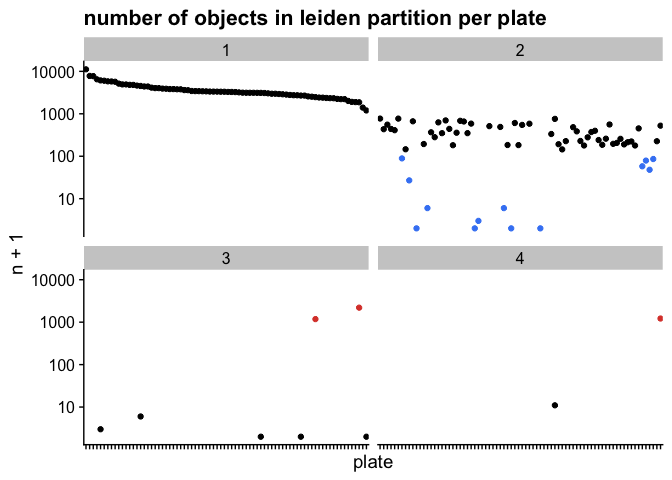
\includegraphics{2.0-nr-embedding_inspection_files/figure-latex/unnamed-chunk-7-1.pdf}

\begin{Shaded}
\begin{Highlighting}[]
\CommentTok{#p2 +  ggsave(paste0(PATH, "notebooks/PhenotypeSpectrum/gg_screen.pdf"), width = 4, height = 4)}
\end{Highlighting}
\end{Shaded}

\begin{Shaded}
\begin{Highlighting}[]
\NormalTok{umap_screen <-}\StringTok{ }\ControlFlowTok{function}\NormalTok{(umap, main)\{}
\NormalTok{  umap }\OperatorTok
\StringTok{  }\CommentTok{#filter(Size < 1000) %>%}
\StringTok{  }\KeywordTok{ggplot}\NormalTok{(}\KeywordTok{aes}\NormalTok{(v1, v2, }\DataTypeTok{color =}\NormalTok{ screen_id)) }\OperatorTok{+}\StringTok{ }
\StringTok{  }\KeywordTok{geom_point_rast}\NormalTok{(}\DataTypeTok{alpha =} \FloatTok{0.5}\NormalTok{, }\DataTypeTok{size =} \FloatTok{0.35}\NormalTok{) }\OperatorTok{+}\StringTok{ }
\StringTok{  }\KeywordTok{scale_color_brewer}\NormalTok{(}\DataTypeTok{type =} \StringTok{"qual"}\NormalTok{) }\OperatorTok{+}\StringTok{ }\CommentTok{#lajolla #vikO}
\StringTok{  }\KeywordTok{theme_cowplot}\NormalTok{() }\OperatorTok{+}
\StringTok{  }\KeywordTok{labs}\NormalTok{(}\DataTypeTok{x =} \StringTok{"UMAP 1"}\NormalTok{,}
       \DataTypeTok{y =} \StringTok{"UMAP 2"}\NormalTok{,}
       \DataTypeTok{title =}\NormalTok{ main,}
       \DataTypeTok{color =} \StringTok{"Screen ID"}\NormalTok{) }\OperatorTok{+}\StringTok{ }
\StringTok{  }\KeywordTok{theme}\NormalTok{(}\DataTypeTok{legend.position =} \StringTok{"bottom"}\NormalTok{)}
\NormalTok{\}}

\NormalTok{p1 <-}\StringTok{ }\KeywordTok{umap_screen}\NormalTok{(umap_sampled_h, }\StringTok{"Harmony normalised, All data"}\NormalTok{)}
\NormalTok{p2 <-}\StringTok{ }\KeywordTok{umap_screen}\NormalTok{(umap_sampled, }\StringTok{"Raw Data, All data"}\NormalTok{)}
\CommentTok{# p3 <- umap_screen(umap_sampled_dmso_h, "Harmony normalised, DMSO")}
\CommentTok{# p4 <- umap_screen(umap_sampled_dmso, "Raw Data, DMSO")}


\KeywordTok{plot_grid}\NormalTok{(}
\NormalTok{  p1, p2,}
\CommentTok{#  p3, p4,}
  \DataTypeTok{labels =} \StringTok{"AUTO"}\NormalTok{, }\DataTypeTok{ncol =} \DecValTok{2}
\NormalTok{) }\OperatorTok{+}\StringTok{  }\KeywordTok{ggsave}\NormalTok{(here}\OperatorTok{::}\KeywordTok{here}\NormalTok{(}\StringTok{"gg_screen_panel.pdf"}\NormalTok{),}
            \DataTypeTok{width =} \DecValTok{8}\NormalTok{,}
            \DataTypeTok{height =} \DecValTok{4}\NormalTok{)}
\end{Highlighting}
\end{Shaded}

\includegraphics{2.0-nr-embedding_inspection_files/figure-latex/unnamed-chunk-8-1.pdf}

\begin{Shaded}
\begin{Highlighting}[]
\CommentTok{#p2 +  ggsave(paste0(PATH, "notebooks/PhenotypeSpectrum/gg_screen.pdf"), width = 4, height = 4)}
\end{Highlighting}
\end{Shaded}

\hypertarget{dye-intensity}{%
\section{Dye Intensity}\label{dye-intensity}}

\begin{Shaded}
\begin{Highlighting}[]
\NormalTok{umap_sampled }\OperatorTok
\StringTok{  }\KeywordTok{ggplot}\NormalTok{(}\KeywordTok{aes}\NormalTok{(actin, }\DataTypeTok{fill =}\NormalTok{ screen_id)) }\OperatorTok{+}
\StringTok{  }\KeywordTok{geom_density}\NormalTok{(}\DataTypeTok{alpha =} \FloatTok{0.5}\NormalTok{) }\OperatorTok{+}\StringTok{ }
\StringTok{  }\KeywordTok{scale_fill_brewer}\NormalTok{(}\DataTypeTok{type =} \StringTok{'qual'}\NormalTok{) }\OperatorTok{+}
\StringTok{  }\KeywordTok{facet_wrap}\NormalTok{(}\OperatorTok{~}\StringTok{ }\NormalTok{line) }\OperatorTok{+}
\StringTok{  }\KeywordTok{theme_cowplot}\NormalTok{()}
\end{Highlighting}
\end{Shaded}

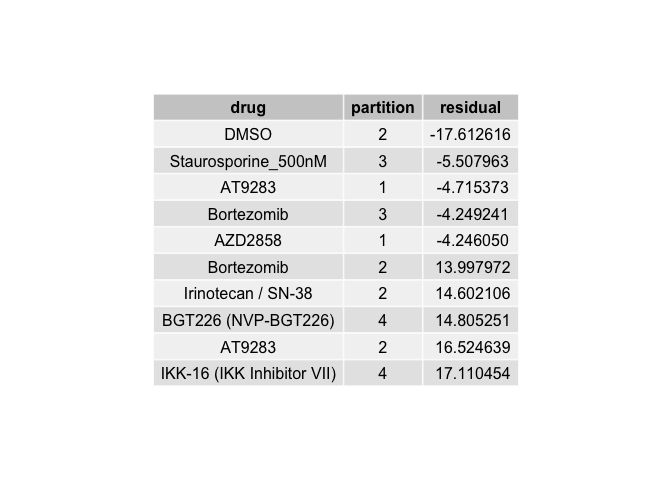
\includegraphics{2.0-nr-embedding_inspection_files/figure-latex/unnamed-chunk-9-1.pdf}

\begin{Shaded}
\begin{Highlighting}[]
\NormalTok{umap_sampled }\OperatorTok
\StringTok{  }\KeywordTok{ggplot}\NormalTok{(}\KeywordTok{aes}\NormalTok{(permeability, }\DataTypeTok{fill =}\NormalTok{ screen_id)) }\OperatorTok{+}
\StringTok{  }\KeywordTok{geom_density}\NormalTok{(}\DataTypeTok{alpha =} \FloatTok{0.5}\NormalTok{) }\OperatorTok{+}\StringTok{ }
\StringTok{  }\KeywordTok{scale_fill_brewer}\NormalTok{(}\DataTypeTok{type =} \StringTok{'qual'}\NormalTok{) }\OperatorTok{+}
\StringTok{  }\KeywordTok{facet_wrap}\NormalTok{(}\OperatorTok{~}\StringTok{ }\NormalTok{line) }\OperatorTok{+}
\StringTok{  }\KeywordTok{theme_cowplot}\NormalTok{()}
\end{Highlighting}
\end{Shaded}

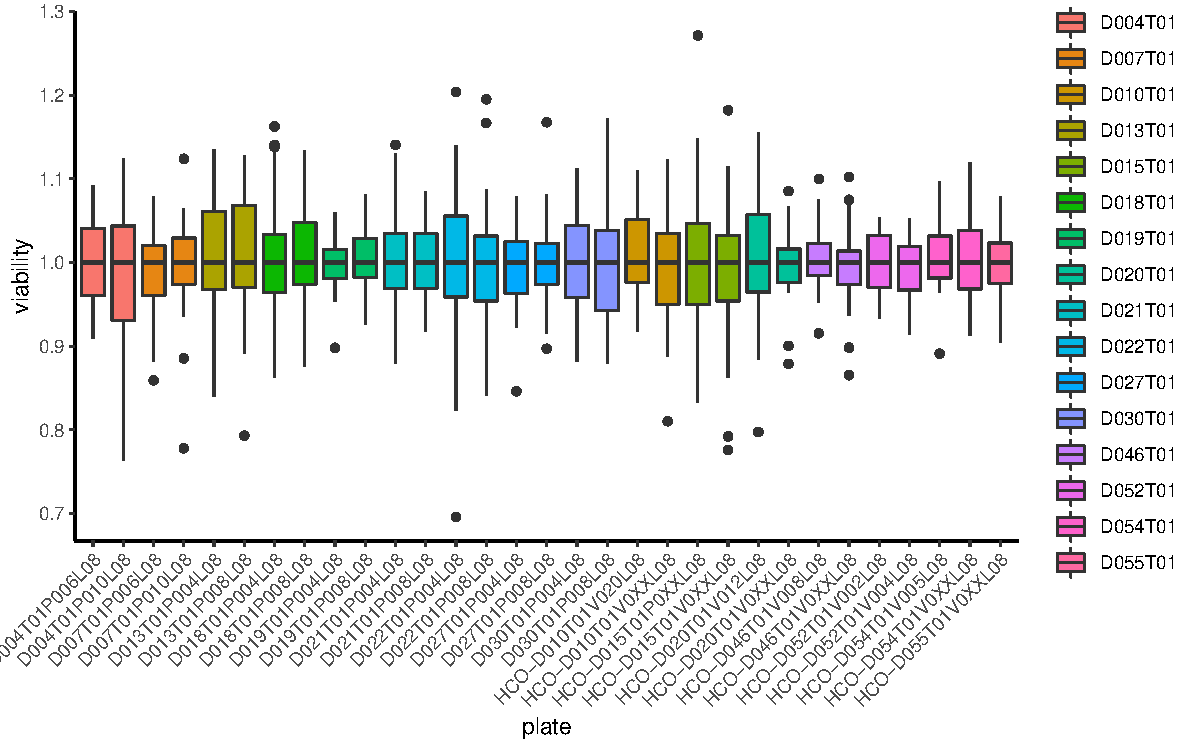
\includegraphics{2.0-nr-embedding_inspection_files/figure-latex/unnamed-chunk-10-1.pdf}

\begin{Shaded}
\begin{Highlighting}[]
\NormalTok{umap_sampled }\OperatorTok
\StringTok{  }\KeywordTok{ggplot}\NormalTok{(}\KeywordTok{aes}\NormalTok{(dapi, }\DataTypeTok{fill =}\NormalTok{ screen_id)) }\OperatorTok{+}
\StringTok{  }\KeywordTok{geom_density}\NormalTok{(}\DataTypeTok{alpha =} \FloatTok{0.5}\NormalTok{) }\OperatorTok{+}\StringTok{ }
\StringTok{  }\KeywordTok{scale_fill_brewer}\NormalTok{(}\DataTypeTok{type =} \StringTok{'qual'}\NormalTok{) }\OperatorTok{+}
\StringTok{  }\KeywordTok{facet_wrap}\NormalTok{(}\OperatorTok{~}\StringTok{ }\NormalTok{line) }\OperatorTok{+}
\StringTok{  }\KeywordTok{theme_cowplot}\NormalTok{()}
\end{Highlighting}
\end{Shaded}

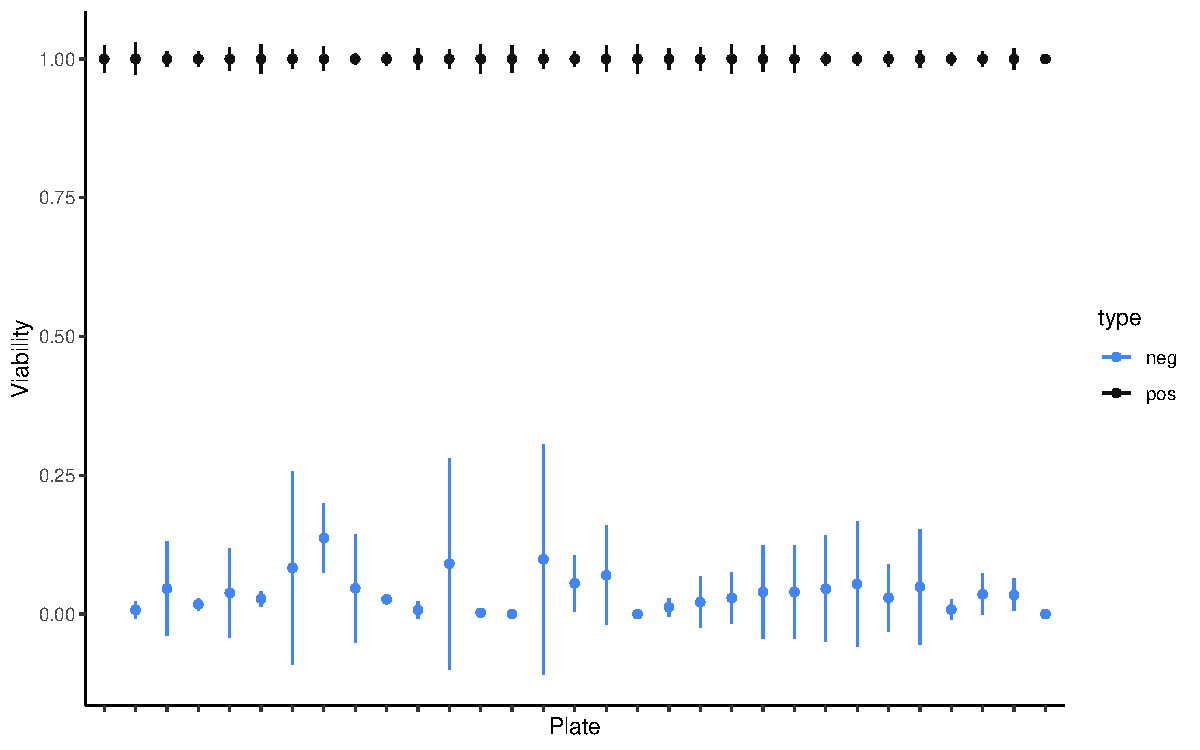
\includegraphics{2.0-nr-embedding_inspection_files/figure-latex/unnamed-chunk-11-1.pdf}

\begin{Shaded}
\begin{Highlighting}[]
\KeywordTok{set.seed}\NormalTok{(}\DecValTok{123}\NormalTok{)}

\NormalTok{umap_sampled }\OperatorTok
\StringTok{  }\KeywordTok{filter}\NormalTok{(drug }\OperatorTok{==}\StringTok{ "DMSO"}\NormalTok{) }\OperatorTok
\StringTok{  }\CommentTok{#sample_n(10000) %>%}
\StringTok{  }\KeywordTok{ggplot}\NormalTok{(}\KeywordTok{aes}\NormalTok{(v1, v2, }\DataTypeTok{color =}\NormalTok{ actin)) }\OperatorTok{+}\StringTok{ }
\StringTok{  }\KeywordTok{geom_point_rast}\NormalTok{(}\DataTypeTok{alpha =} \FloatTok{0.75}\NormalTok{, }\DataTypeTok{size =} \FloatTok{0.35}\NormalTok{) }\OperatorTok{+}
\StringTok{   }\KeywordTok{scale_colour_gradient}\NormalTok{(}\DataTypeTok{low =} \StringTok{"white"}\NormalTok{, }\DataTypeTok{high =} \StringTok{"red"}\NormalTok{) }\OperatorTok{+}\StringTok{ }
\StringTok{  }\KeywordTok{theme_cowplot}\NormalTok{() }\OperatorTok{+}
\StringTok{  }\KeywordTok{labs}\NormalTok{(}\DataTypeTok{x =} \StringTok{"UMAP 1"}\NormalTok{,}
       \DataTypeTok{y =} \StringTok{"UMAP 2"}\NormalTok{,}
       \DataTypeTok{title =} \StringTok{"Actin staining intensity"}\NormalTok{) }\OperatorTok{+}\StringTok{ }
\StringTok{  }\KeywordTok{theme}\NormalTok{(}\DataTypeTok{legend.position =} \StringTok{"bottom"}\NormalTok{) }\OperatorTok{+}\StringTok{ }
\StringTok{  }\KeywordTok{ggsave}\NormalTok{(here}\OperatorTok{::}\KeywordTok{here}\NormalTok{(}\StringTok{"reports/figures/gg_actin.pdf"}\NormalTok{), }\DataTypeTok{width =} \DecValTok{4}\NormalTok{, }\DataTypeTok{height =} \DecValTok{4}\NormalTok{)}
\end{Highlighting}
\end{Shaded}

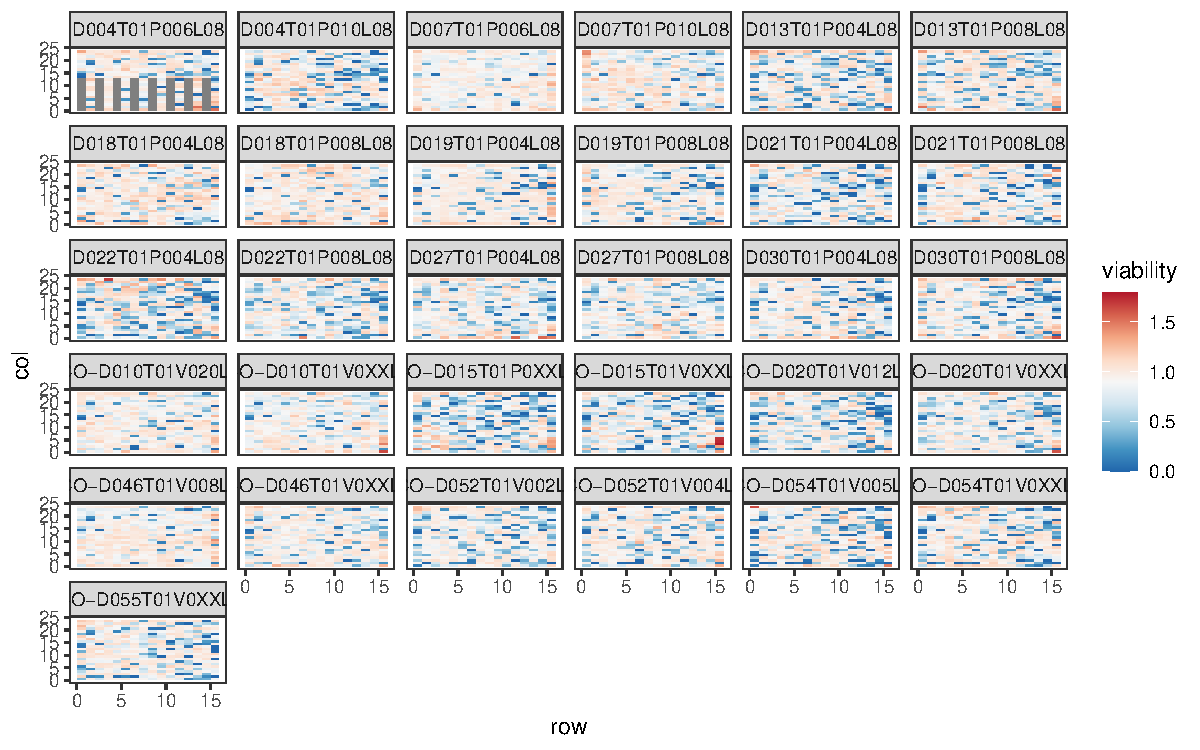
\includegraphics{2.0-nr-embedding_inspection_files/figure-latex/unnamed-chunk-12-1.pdf}

\begin{Shaded}
\begin{Highlighting}[]
\NormalTok{umap_sampled }\OperatorTok
\StringTok{  }\KeywordTok{filter}\NormalTok{(drug }\OperatorTok{==}\StringTok{ "DMSO"}\NormalTok{) }\OperatorTok
\StringTok{  }\CommentTok{#sample_n(10000) %>%}
\StringTok{  }\KeywordTok{ggplot}\NormalTok{(}\KeywordTok{aes}\NormalTok{(v1, v2, }\DataTypeTok{color =}\NormalTok{ dapi)) }\OperatorTok{+}\StringTok{ }
\StringTok{  }\KeywordTok{geom_point_rast}\NormalTok{(}\DataTypeTok{alpha =} \FloatTok{0.75}\NormalTok{, }\DataTypeTok{size =} \FloatTok{0.35}\NormalTok{) }\OperatorTok{+}
\StringTok{   }\KeywordTok{scale_colour_gradient}\NormalTok{(}\DataTypeTok{low =} \StringTok{"white"}\NormalTok{, }\DataTypeTok{high =} \StringTok{"blue"}\NormalTok{) }\OperatorTok{+}\StringTok{ }
\StringTok{  }\KeywordTok{theme_cowplot}\NormalTok{() }\OperatorTok{+}
\StringTok{  }\KeywordTok{labs}\NormalTok{(}\DataTypeTok{x =} \StringTok{"UMAP 1"}\NormalTok{,}
       \DataTypeTok{y =} \StringTok{"UMAP 2"}\NormalTok{,}
       \DataTypeTok{title =} \StringTok{"Nuclear staining intensity"}\NormalTok{) }\OperatorTok{+}\StringTok{ }
\StringTok{  }\KeywordTok{theme}\NormalTok{(}\DataTypeTok{legend.position =} \StringTok{"bottom"}\NormalTok{) }\OperatorTok{+}\StringTok{ }
\StringTok{  }\KeywordTok{ggsave}\NormalTok{(here}\OperatorTok{::}\KeywordTok{here}\NormalTok{(}\StringTok{"reports/figures/gg_dapi.pdf"}\NormalTok{), }\DataTypeTok{width =} \DecValTok{4}\NormalTok{, }\DataTypeTok{height =} \DecValTok{4}\NormalTok{)}
\end{Highlighting}
\end{Shaded}

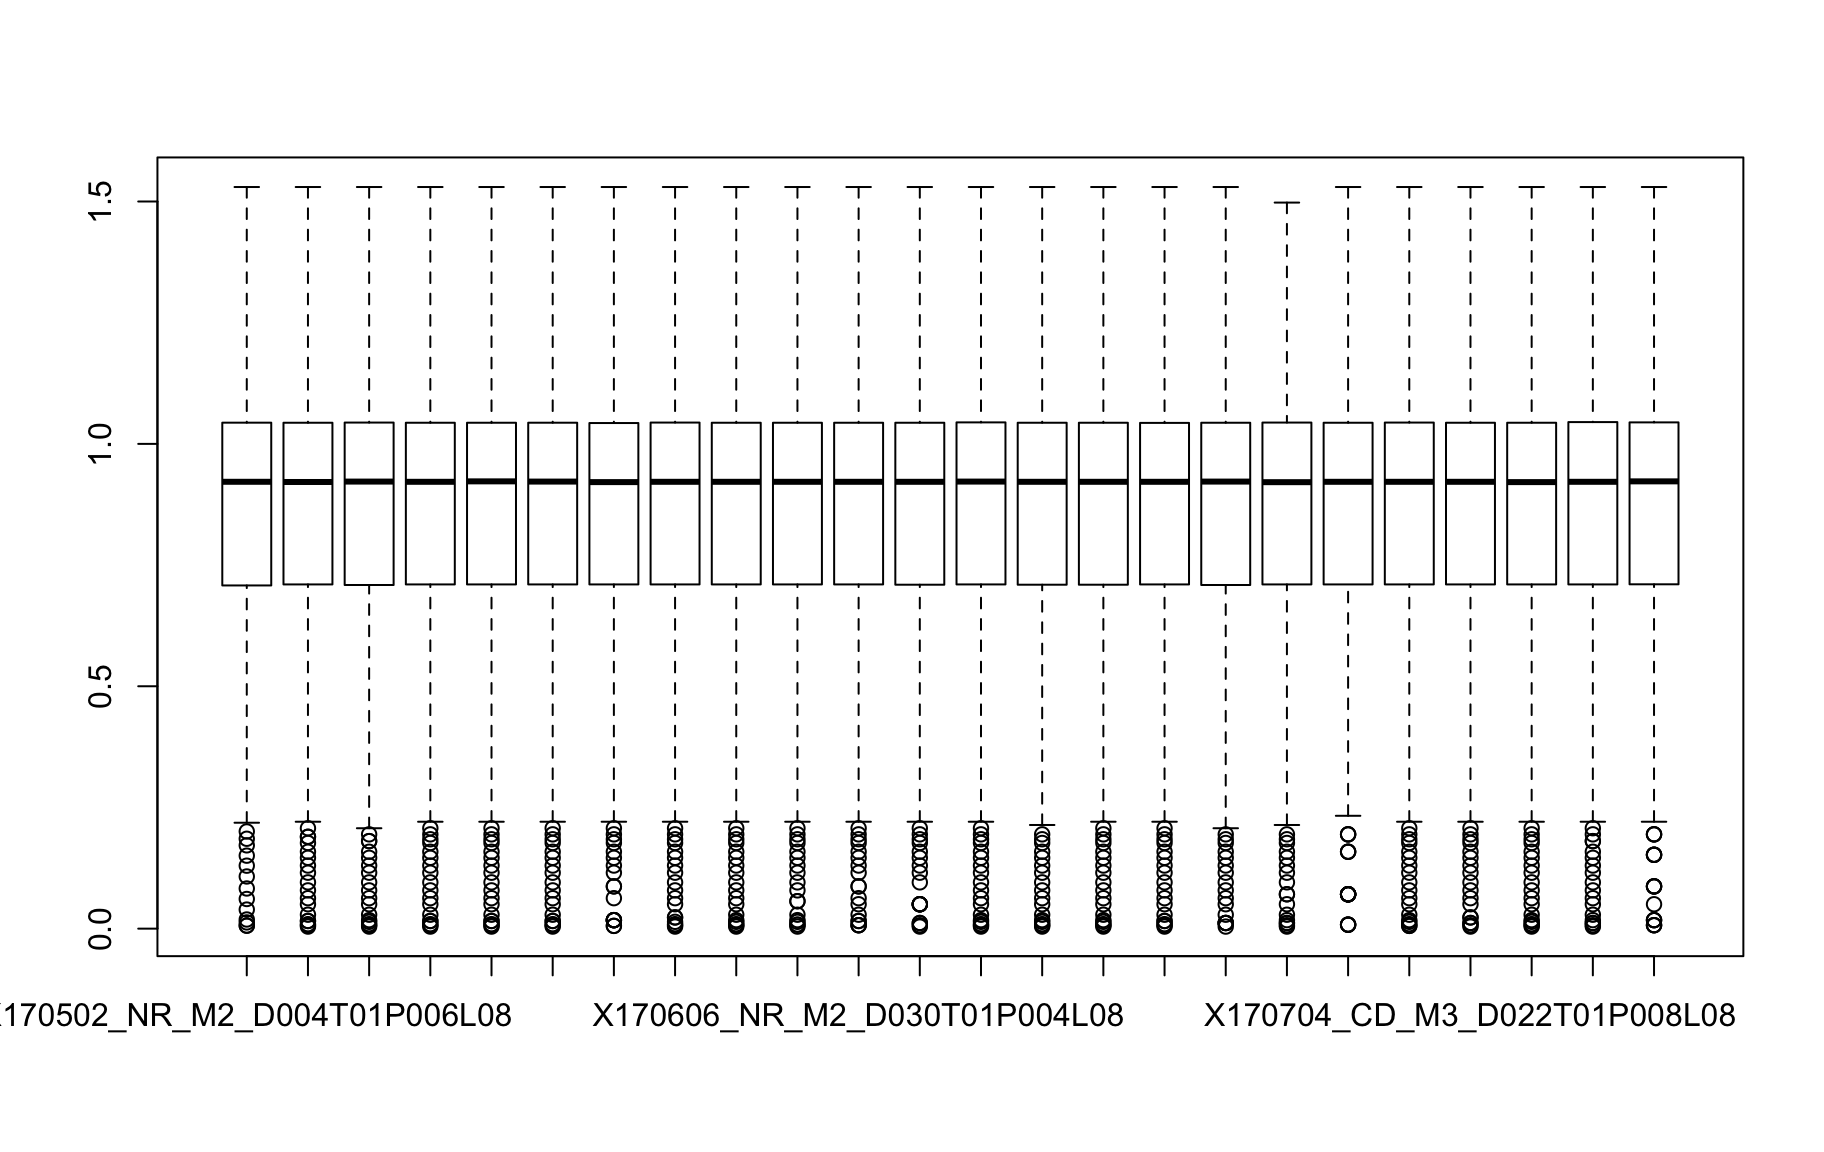
\includegraphics{2.0-nr-embedding_inspection_files/figure-latex/unnamed-chunk-12-2.pdf}

\hypertarget{supplements}{%
\section{Supplements}\label{supplements}}

Here I collect pieces of code that did not make it into the final
analysis but can be run in theory. In order to access these peaces of
code, you have to open the \emph{.RMD} file.

\begin{Shaded}
\begin{Highlighting}[]
\NormalTok{knitr}\OperatorTok{::}\KeywordTok{knit_exit}\NormalTok{()}
\end{Highlighting}
\end{Shaded}

\end{document}
